\documentclass[12pt, letterpaper]{article}

\usepackage[margin=1in]{geometry}
\usepackage{graphicx}
\usepackage{float}
\usepackage{parskip}
\usepackage{amsmath}
\usepackage[T1]{fontenc}
\usepackage{lmodern}
\usepackage{hyperref}

\graphicspath{{images/}}

\title{\textbf{Servo Deployment Mechanism:\\Circuit Design and Justification}}
\author{ESC204, Engineering Science Praxis III \\ University of Toronto}
\date{March 2026}

\begin{document}
\maketitle
\tableofcontents
\newpage

% ============================================================
\section{Overview}

The sensor-box deployment system uses two servomotors: a TowerPro MG996R to drive linear
actuation of the deployment arm, and a DFRobot DF9GMS to rotate a keyed shaft that latches
onto the sensor box extrusion. This document justifies the selection and circuit design for
each servo, drawing on their respective datasheets [2][3] and the servo characterisation
work from Lab 4 [1].

% ============================================================
\section{Deployment Strategy}

\subsection{MG996R: Linear Actuation}

The deployment arm requires a linear stroke. Since servomotors produce rotational output, a
lever linkage converts the MG996R's angular sweep ($0°$ to $180°$) into the required linear
travel. The MG996R is selected for this role based on its high stall torque of 9.4\,kg$\cdot$cm
at 4.8\,V and 11\,kg$\cdot$cm at 6\,V [2], which provides the force margin needed to move
the arm against inertial and frictional loads. Its metal gear construction [2] also makes it
suitable for the sustained mechanical loading of a deployment stroke. The operating voltage
range of 4.8\,V to 7.2\,V [2] is comfortably met by the 5\,V regulated supply described in
Section~\ref{sec:circuit}.

Wire connections for the MG996R are: brown to GND, red to VCC (5\,V), and orange to the
Pico PWM signal pin [2].

\subsection{DF9GMS: Latch Key}

Once the arm is fully extended, the DF9GMS rotates the latch key through a limited angle to
engage the sensor box extrusion. At a stall torque of 1.6\,kg$\cdot$cm and a weight of
only 9\,g [3], the DF9GMS is well suited to this low-load, precision task: it is
approximately 6$\times$ lighter than the MG996R (55\,g [2]), minimising the mass added to
the latch sub-assembly. Its 0.5\,ms deadband width [3] provides repeatable positioning,
sufficient for reliable latch engagement. The DF9GMS operates over the same 4.8\,V to 6\,V
range [3] as the shared 5\,V supply.

Wire connections for the DF9GMS are: brown to GND, red to VCC (5\,V), and orange to the
Pico PWM signal pin [3].

The deployment sequence is software-enforced: the DF9GMS latch servo only fires after the
MG996R has completed its stroke, preventing mechanical interference.

% ============================================================
\section{Circuit Design}
\label{sec:circuit}

\subsection{Power and Wiring}

Both servos require 4.8\,V to 6\,V, while the Pico outputs only 3.3\,V, insufficient to
power either servo. An external 12\,V supply steps down to 5\,V via the L298N motor
driver's onboard regulator, consistent with the Lab 4 validated approach [1]. The L298N
driver outputs are not used; it functions purely as a 5\,V regulator. Key wiring rules:

\begin{itemize}
    \item Both servo VCC and GND wires connect to the L298N 5\,V output and common ground.
    \item Each servo's orange signal wire connects to a dedicated Pico GPIO pin configured
          as a PWM output. The 3.3\,V logic level is compatible with standard servo signal
          inputs, as confirmed in Lab 4 [1].
    \item All grounds (Pico, L298N, both servos, 12\,V supply) share a common node.
    \item The Pico is powered separately via USB and is never connected to the 5\,V or 12\,V rails.
\end{itemize}

\subsection{PWM Control}

Both the MG996R and DF9GMS use the standard RC servo PWM protocol: a 50\,Hz signal
(20\,ms period) with pulse width encoding the target angle [2][3]:

\begin{itemize}
    \item 1\,ms $\approx 0°$
    \item 1.5\,ms $\approx 90°$
    \item 2\,ms $\approx 180°$
\end{itemize}

The Pico's hardware PWM peripheral generates the signal on each dedicated GPIO pin. The
duty cycle is computed as:
\[
    \text{duty} = \frac{t_{\text{pulse}}}{20\,\text{ms}} \times 65535
\]
Since both servos share the same PWM protocol, the firmware uses a common servo control
function parameterised by pin number and target angle, with separate calls for each servo.

\subsection{Circuit Diagrams and Two-Servo Scaling}

The diagrams in Figures~\ref{fig:schematic} and~\ref{fig:layout} depict the single-servo
characterisation circuit from Lab 4 [1]. The two-servo deployment circuit is a direct
extension: both servos share the same 5\,V and GND rails, with each signal wire routed to a
separate Pico GPIO pin. No additional power components are required, since the L298N
regulator output is sufficient to supply both servos. To stay within the regulator's thermal
limits, the PWM signals are staggered in time, which is already satisfied by the sequenced
deployment logic in Section 2. Since power and control are fully independent per servo,
adding the second servo is purely additive.

\begin{figure}[H]
    \centering
    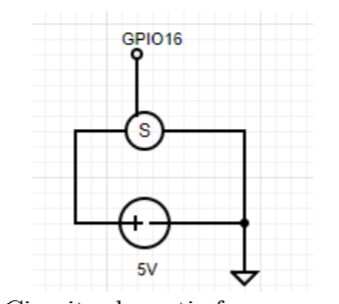
\includegraphics[width=0.60\textwidth]{circuit_schematic.png}
    \caption{Circuit schematic (single-servo reference from Lab 4 [1]). For the two-servo
             deployment system, the second servo's VCC and GND connect to the same 5\,V
             rail, with its signal wire on a separate Pico GPIO pin.}
    \label{fig:schematic}
\end{figure}

\begin{figure}[H]
    \centering
    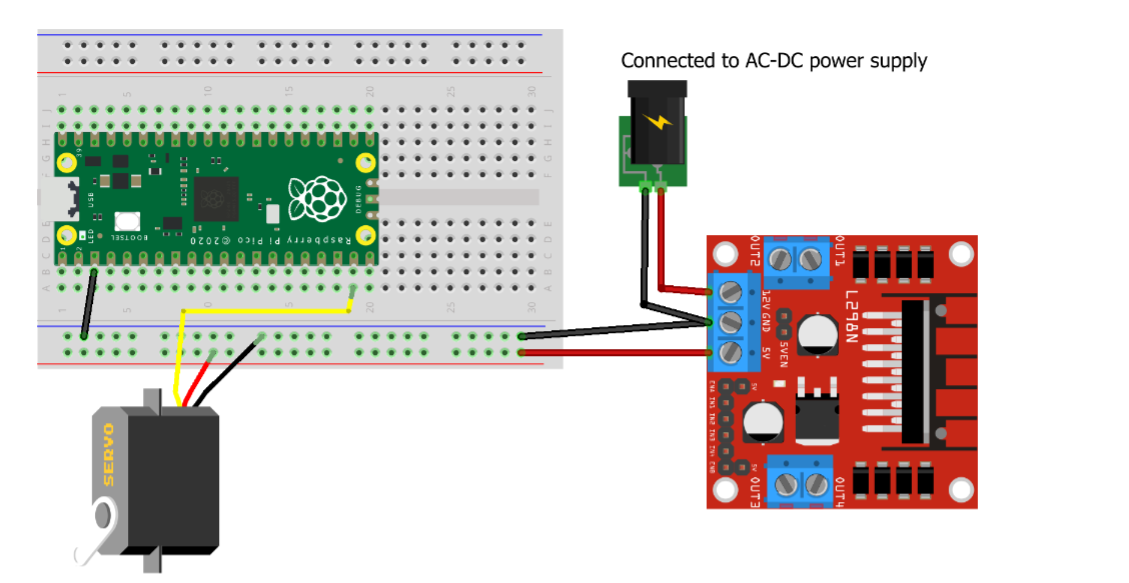
\includegraphics[width=0.75\textwidth]{circuit_layout.png}
    \caption{Physical board layout (single-servo reference). The second servo is wired
             identically: power from the shared 5\,V/GND rail, signal to an additional
             Pico GPIO pin.}
    \label{fig:layout}
\end{figure}

% ============================================================
\section{Operational Notes}

\textbf{Thermal management:} The L298N regulator can overheat under sustained load [1].
The MG996R draws up to 2.5\,A at stall [2], so once each servo reaches its target position,
the PWM signal is held constant so the servo maintains position without drawing continuous
stall current.

\textbf{Pre-power checklist (adapted from Lab 4 [1]):}
\begin{itemize}
    \item Confirm L298N 5\,V rail reads $5.0 \pm 0.25$\,V with a DMM.
    \item Confirm all grounds are common.
    \item Confirm no shorts across power rails before connecting 12\,V.
\end{itemize}

% ============================================================
\section{Conclusion}

The MG996R and DF9GMS are well matched to their respective roles. The MG996R's high stall
torque (up to 11\,kg$\cdot$cm at 6\,V [2]) handles the mechanical demand of linear arm
actuation, while the DF9GMS's low mass (9\,g [3]) and sufficient torque (1.6\,kg$\cdot$cm
[3]) make it ideal for the precision latch key motion. Both operate over the same 5\,V
supply rail and use identical PWM protocols, so the two-servo circuit requires no additional
power hardware beyond the single-servo Lab 4 reference design. Sequenced software control
keeps thermal load within safe limits and ensures reliable, repeatable deployment.


\newpage
% ============================================================
\begin{thebibliography}{9}

\bibitem{lab4}
University of Toronto Engineering Science,
\textit{ESC204S Winter 2026 Lab 4 Instructions},
Version 1.0, January 29, 2026.

\bibitem{mg996r}
TowerPro,
\textit{MG996R Metal Gear Servo Datasheet},
[Online]. Available: \url{https://components101.com/sites/default/files/component_datasheet/MG996R-Datasheet.pdf}

\bibitem{df9gms}
DFRobot,
\textit{DF9GMS 180° Micro Servo Product Page},
[Online]. Available: \url{https://www.dfrobot.com/product-255.html}

\end{thebibliography}

\end{document}
